\section{The \toolname{} Workflow}
\label{sec:overview}

In this section, we give an overview of the workflow used in \toolname{} using the \texttt{RingBuffer}~(\Cref{ex:rb}) as a running example.

%\paragraph{Input and Output}
The input to \toolname{} consists of two parts: (1) a user-provided Rust implementation of the code to be verified (e.g., the code in \Cref{fig:ring-buffer-verified} but \emph{without} any annotations---the green-highlighted lines would be absent), and (2) a unit-test suite that conveys typical usage patterns and rules out trivial specifications. The output is a fully annotated version of the code that passes the Verus verifier (e.g., the full \texttt{RingBuffer} code as shown in \Cref{fig:ring-buffer-verified}). Care is taken to ensure that both the code and the tests remain unchanged throughout the workflow.
%Below we detail how \toolname{} translates the original Rust implementation into a verified artifact.

\begin{figure}[t]
  \centering
  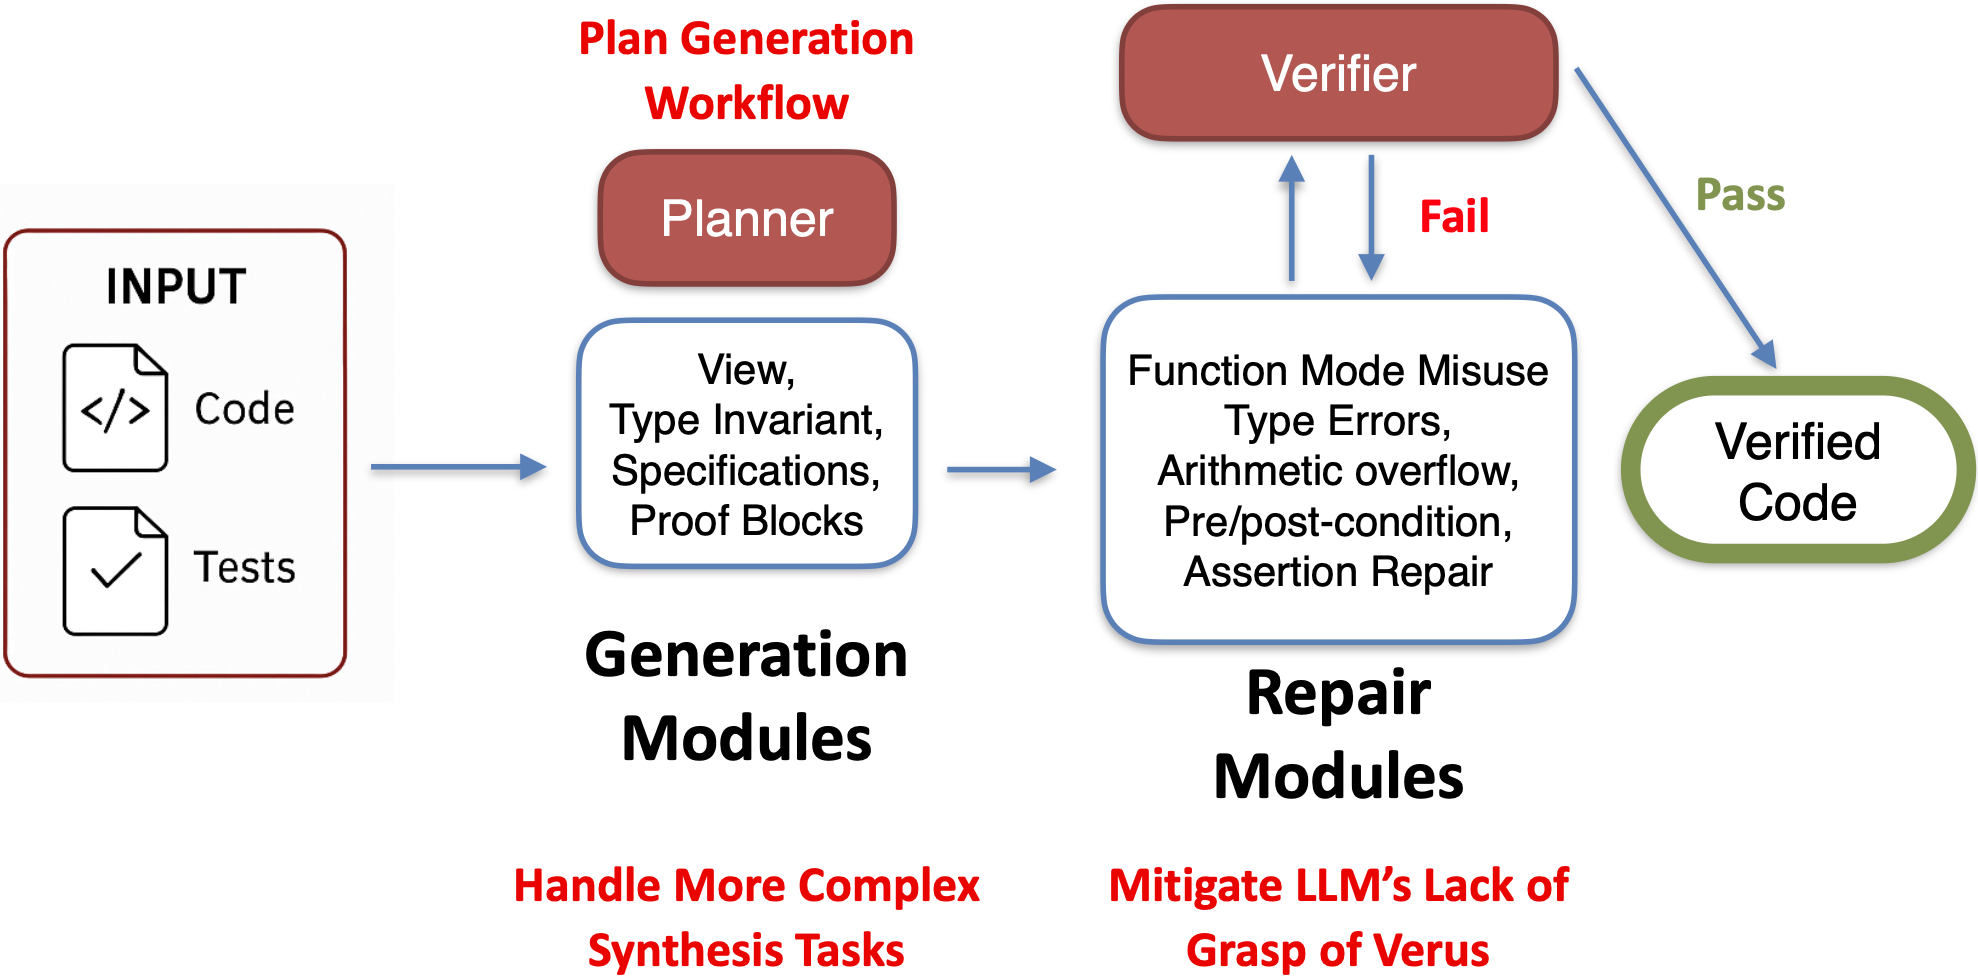
\includegraphics[width=\textwidth]{workflow-new.png}
  \caption{Workflow of \toolname{}, where rounded rectangles denote modules} %Rounded rectangles denote file artifacts (test cases, source files, verified outputs) while plain rectangles denote workflow steps; diamonds indicate decisions.
%  }
  \label{fig:workflow}
\end{figure}


The overall workflow is shown in \Cref{fig:workflow}. \toolname{} builds on the general approach of the AutoVerus system~\cite{autoverus}, in that it consists of a network of modules that collaborate to complete program verification tasks. However, as noted in the challenge discussion of \Cref{sec:intro}, verifying data structures requires techniques and components not found in AutoVerus or any prior work~\cite{autoverus,cav24llm,classinvgen,dafnysinglemethod,dafny-annotator}.

\begin{small}
\begin{algorithm}[htbp]
\SetAlgoNoLine 
\SetKwProg{Fn}{Function}{}{end}
\caption{The Outermost Algorithm of \toolname{}}
\label{fig:outmost}
\textbf{Input.} {\texttt{code}: the data structure code to be verified; \texttt{test}: unit test suite}\\
\textbf{Output.} {verified version of \texttt{code}}\\
\Fn{{{\rm \textbf{VerifyModule}}}{\rm (}{\tt code}, {\tt test}{\rm )}}{
{\tt code} $\gets$ \genfunc{}({\tt code}, {\tt test}) \textcolor{gray}{// Stage 1: Generate the Annotations}\\
\Return \fixfunc{}({\tt code}, {\tt test}) \textcolor{gray}{// Stage 2: Repair Annotations}\\
}
\end{algorithm}
\end{small}

\toolname{} applies a two-stage pipeline as shown in \Cref{fig:outmost} to synthesize annotations and perform verification.
\begin{enumerate}
\item Stage 1: Generate the initial draft of annotations through the function \genfunc{}. The detailed process is described in \Cref{sec:genfunc}.
\item Stage 2: Invoke \fixfunc{} to iteratively detect and repair incorrect annotations. The details are presented in \Cref{sec:fixfunc}.
\end{enumerate}

\noindent
Due to space limitations, we only present sketches of our prompts, but the full details of our prompts are publicly available~\cite{artifact}.



%Each stage consists of several modules with dedicated usage.





